\section{Digital filtrering}
Der findes to former for digital filtrering; Infinite Impulse Response (IIR) og Finite Impulse Response (FIR). Der ses hertil både fordele og ulemper ved begge filtertyper \citep{blandford2012}.

FIR-filtre kan altid laves, således de har en lineær fase, og de er altid stabile. FIR-filtre designes ved at benytte eksempelvis frekvenssampling eller en bestemt vindue-type, hvilket giver en overførselsfunktion. Denne overførselsfunktion kan herved benyttes som digitalt filter \citep{blandford2012}. 

I modsætning til FIR-filtre, har IIR-filtre ikke en lineær fase, og de kan være ustabile. Ud over dette har IIR-filtre stejlere sidelobes end et IIR-filter med samme antal koefficienter. Dette betyder, at filteret er mindre hukommelseskrævende og kan arbejde hurtigere. IIR-filtres designprocedure er udledt af den procedure, som de analoge filtre er designet efter. Af denne grund laves IIR-filtre, ligesom analoge filtre, som Butterworth, Chebyshev type 1 og 2 og elliptiske filtre \citep{blandford2012}. Disse er illustreret på \autoref{fig:filtre}. 
\\

\begin{figure}[H]
\centering
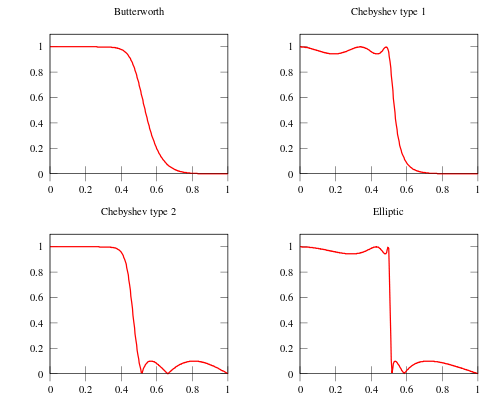
\includegraphics[width=0.6\textwidth]{figures/filtre}
\caption{De fire filtertyper; Butterworth, Chebyshev 1 \& 2 og elliptisk \citep{wikipedia2016}}
\label{fig:filtre}
\end{figure}

\noindent
Et Butterworth filter er karakteriseret ved ikke at have nogle rippels i hverken pasbåndet eller stopbåndet. Hertil er der, uanset filterorden, en dæmpning på 3 dB ved knækfrekvensen \citep{nilsson2015}.
Et Chebyshev filter har i modsætning til Butterworth et kortere transitionsbånd, som følge af en stejlere dæmpning, dog forekommer der ved et Chebyshev filter enten rippels i pasbåndet eller i stopbåndet. Ved et type 1 Chebyshev filter ses rippels i pasbåndet samt en monotont variation i stopbåndet. For type 2 Chebyshev ses der derimod rippels i stopbåndet og en monotont variation i pasbåndet \citep{nilsson2015}. 
Ved det elliptiske filter ses en endnu stejlere dæmpning og dermed et kortere transitionsbånd end ved Butterworth samt Chebyshev filtre. Ved dette filter ses der dog både rippels i pasbånd og stopbånd \citep{nilsson2015}. 

\vspace{3mm}
\noindent
Et moving average filter er et simpelt lavpas FIR filter, der oftest anvendes til at smoothe et array af data, der er samplet. Der kan vælges forskellig filterlængde ved implementeringen af filteret. Et moving average filter kan betragtes som et vindue af en bestemt størrelse, der bevæger sig henad et array med ét element ad gangen. Det midterste værdi i vinduet vil  erstattes med gennemsnitsværdien for de data, der er i vinduet. Den midsterste værdi i vinduen må dog ikke erstattes med gennemsnitsværdien før vinduet har passeret, således alle gennemsnitsværdier er baseret på de originale data. Det er derfor vigtigt at huske på de beregnede gennemsnitværdier.  af \autoref{fig:maf} ses et vindue, der i dette tilfælde har en størrelse på 8. Her tages gennemsnittet for de 8 værdier i vinduet, hvorefter denne værdi erstatter væriden på den 4. plads i vinduet.\citep{atmel2002}

begin{figure} [H]
\centering
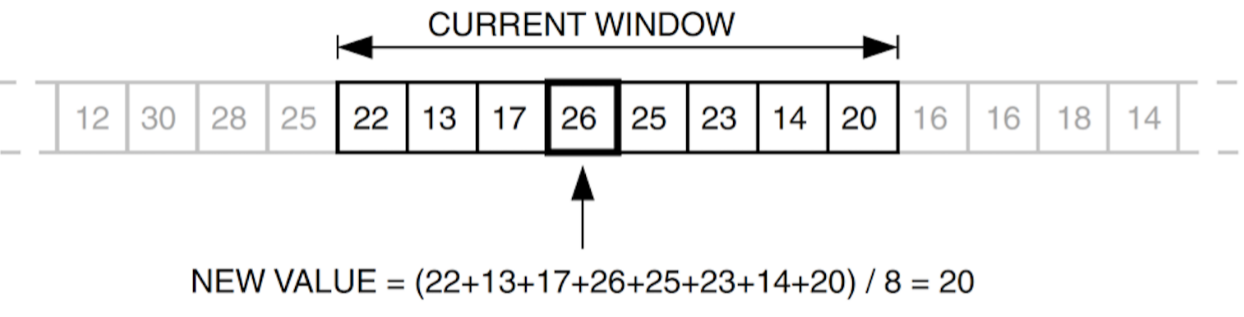
\includegraphics[width=0.8\textwidth]{figures/maf}
\caption{Gennemsnitsværdien beregnes for et vindue for et moving average filter}.}
\label{fig:maf}
\end{figure} 

Af \autoref{eq:mafl} fremgår formlen for udregingen af et moving average filter. 
\begin{equation}
y[i]=\dfrac{1}{M}\sum^{M-1}_{j=0} x[i-j]
\label{eq:mafl}
\end{equation}

\subsubsection{Filtrering af EMG-signal}
Under pilotforsøget i \autoref{sec:pilotforsoeg} kunne det ses, at udglatningen af signalet fra det analoge envelopefilter ikke er tilstrækkeligt i forhold til, at signalet skal få et exoskelet til at bevæge sig efter en patients ben. Da der derfor ønskes at frafiltrere yderligere højfrekvent støj fra det forstærkede, ensrettede og lavpasfiltrerede EMG-signal, vil et IIR-lavpasfilter være fordelagtigt at implementere, da et FIR-filter kræve for meget af PSoC'en. Dette andet, og digitale, lavpasfilter skal fungere som endnu et envelopefilter, så signalet bliver yderligere udglattet, men det skal stadig følge muskelsignalet, så det ikke bliver uhensigtmæssigt svært at aktivere exoskelettet.  
Af denne grund testes forskellige filterdesigns på resultaterne fra pilotforsøget. Dette indebærer, at forskellige knækfrekvenser og filterordener undersøges for at teste, hvordan disse valg påvirker signalet. På denne måde bliver det muligt at beslutte, hvordan filteret skal designes, og hvilke krav der skal opstilles. Filtrene designes som Butterworth-konfigurationer, da der ønskes maksimal fladhed i både pas-, transistions- og stopbånd. 

Først vælges filterets knækfrevkens ved at afprøve flere forskellige. Eksempler på disse knækfrekvenser ses på \ref{fig:lp_knaek}, hvor $15~Hz$, $20~Hz$ og $25~Hz$ er repræsenteret. 

\begin{figure} [H]
\centering
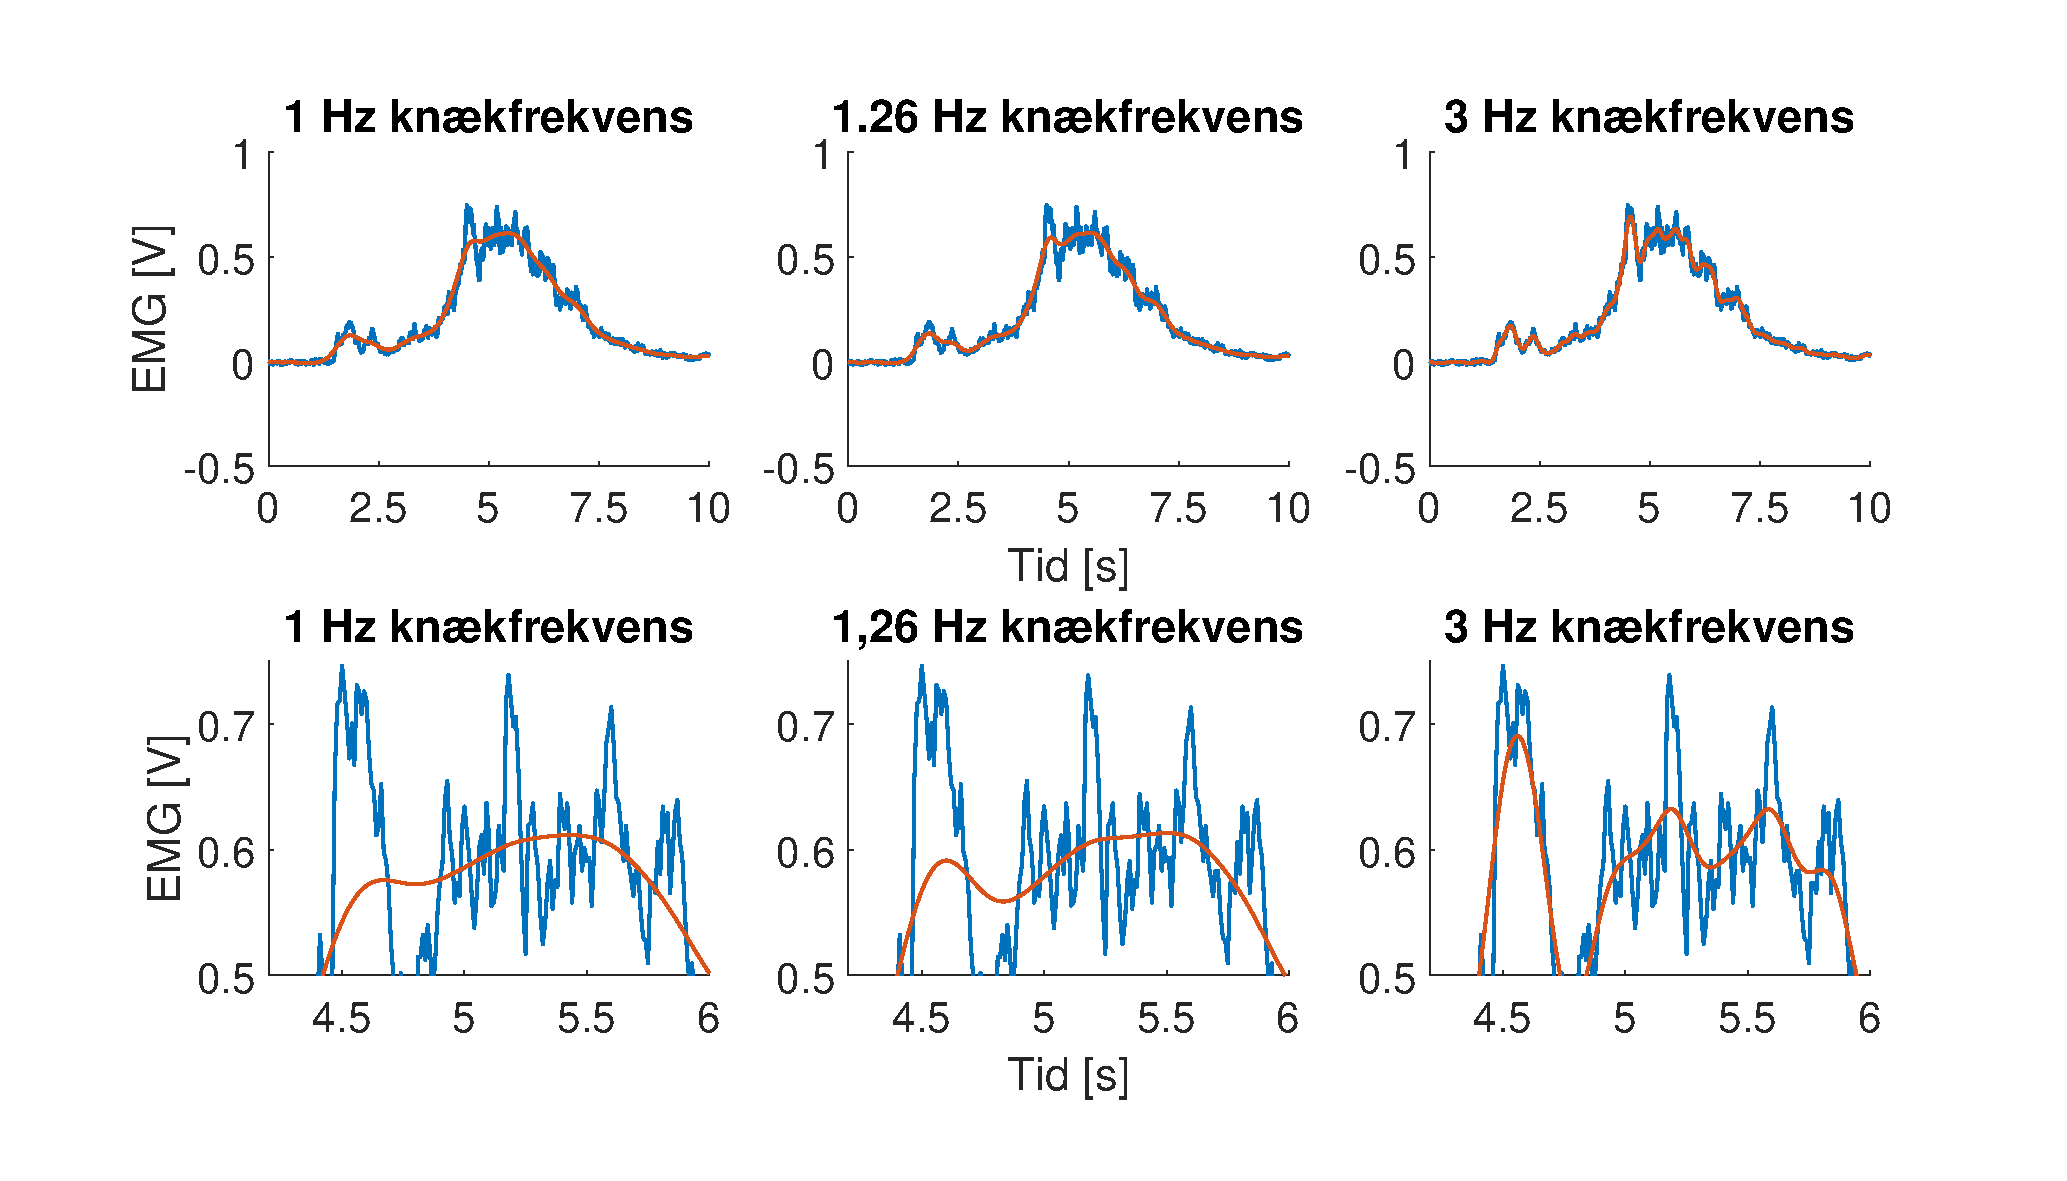
\includegraphics[width=1\textwidth]{figures/problemloesning/lavpas_knaek}
\caption{De blå grafer viser resultater fra pilotforsøget. De røde linjer på hver graf viser lavpasfiltre med knækfrekvenser på hhv. 15, 20 og $25~Hz$.}
\label{fig:lp_knaek}
\end{figure} 

\noindent
Ud fra \ref{fig:lp_knaek} vælges en knækfrekvens på $20~Hz$, da denne følger signalet samtidigt med at udglatte spikes, der vil kunne forstyrre signalet til exoskelettet, hvilket de to andre knækfrekvenser ikke formår at gøre.

Herefter bestemmes, på samme måde som ved knækfrekvensen, hvilken filterorden der vil være mest optimal til filteret. 

\begin{figure} [H]
\centering
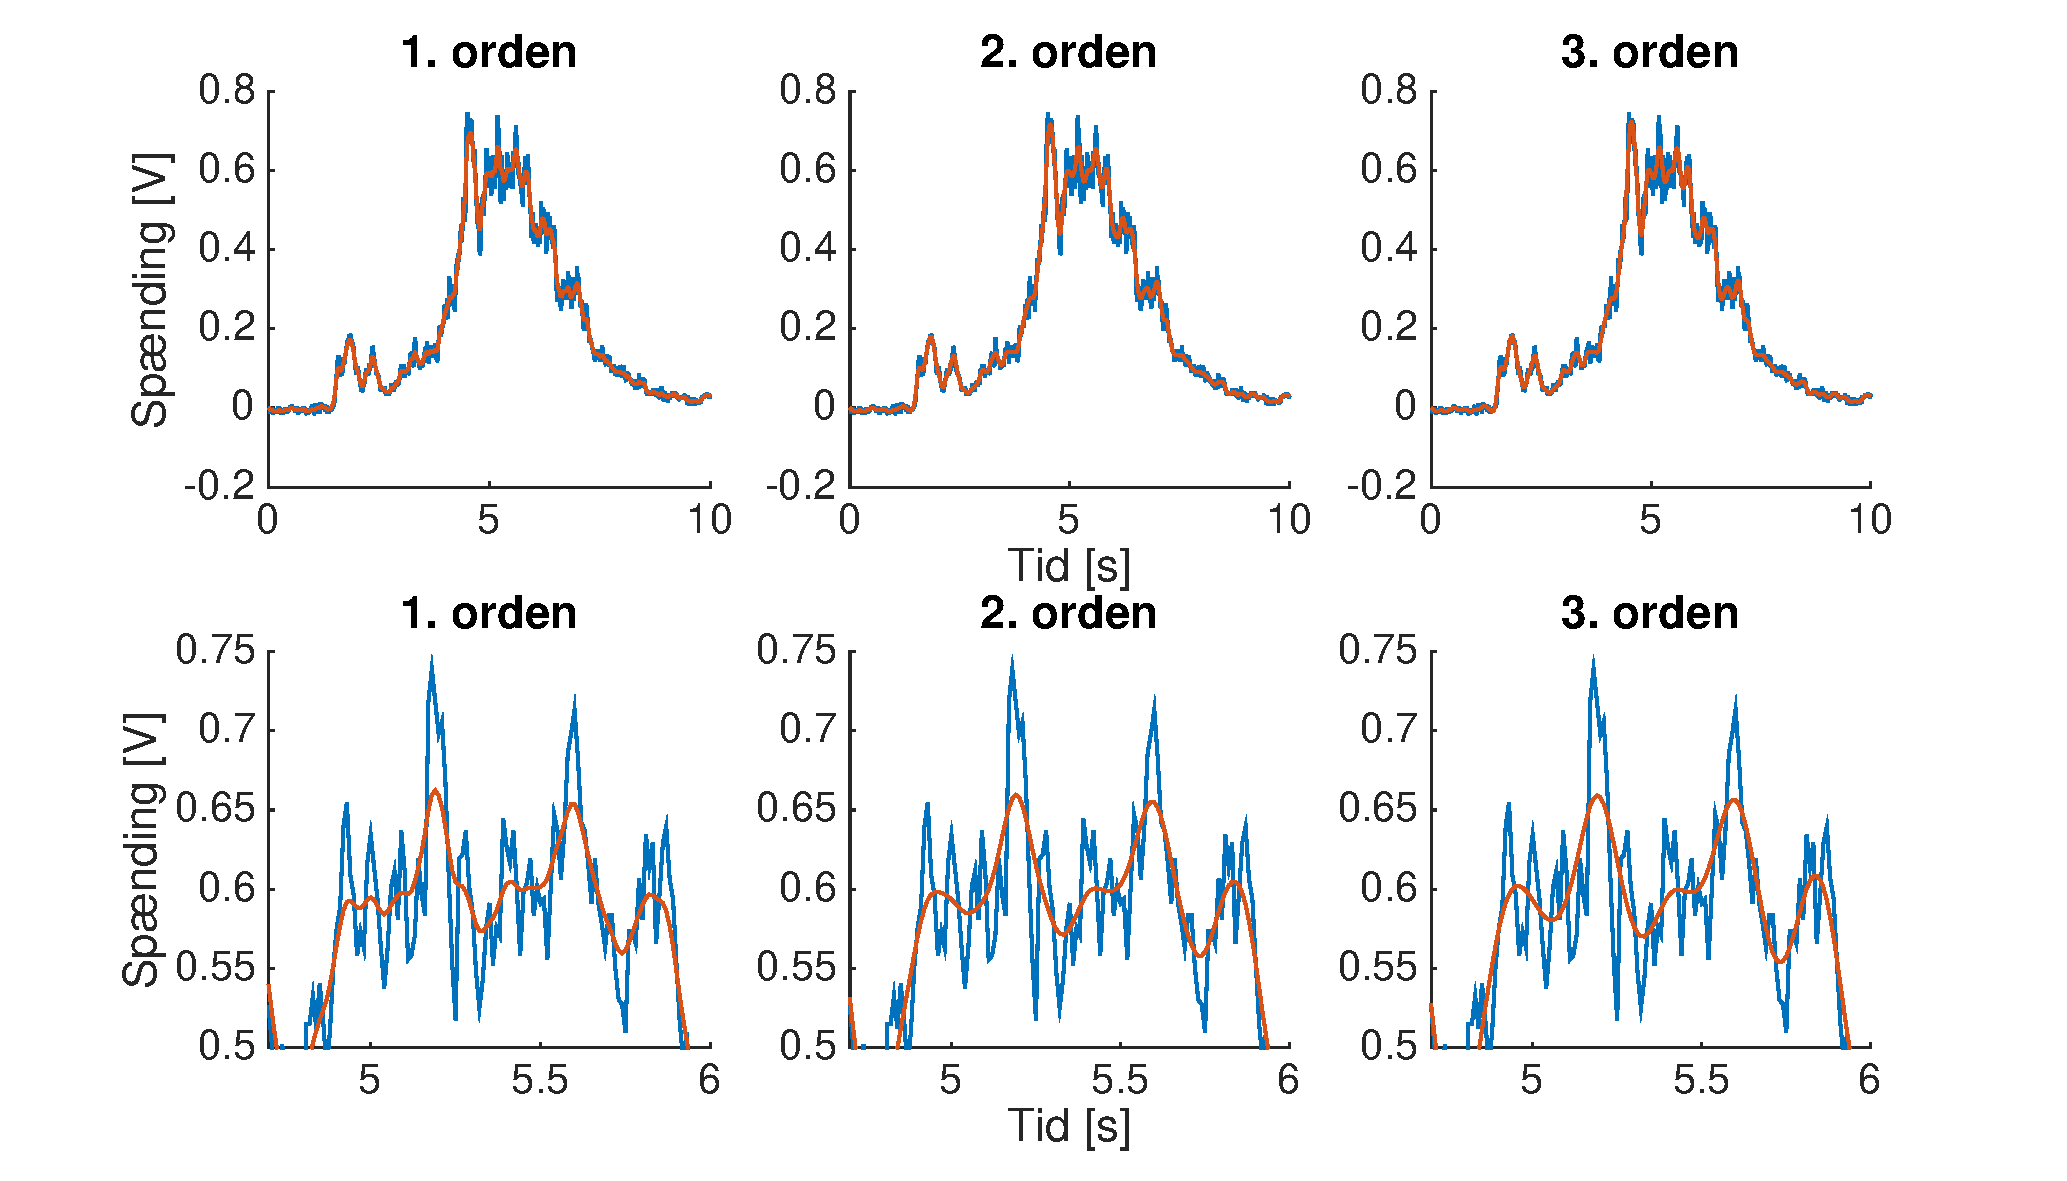
\includegraphics[width=1\textwidth]{figures/problemloesning/lavpas_orden}
\caption{De blå grafer viser resultater fra pilotforsøget. De røde linjer på hver graf viser lavpasfiltre med filterordner på hhv. 1, 2 og 3.}
\label{fig:lp_orden}
\end{figure} 

\noindent
Ud fra \ref{fig:lp_orden} vælges en filterorden på 2, da denne vurderes til være tilstrækkelig. Der ses ingen større forskel i outputsignalet fra filteret, hvis filterordenen hæves yderligere. Dertil vurderes det, at en filterorden på 1 ikke er tilstrækkelig, da dette filters outputsignal afviger for meget fra inputsignalet. 

\vspace{3mm}

\textbf{Krav:}
\begin{itemize}
\item Skal stabiliseres signalets amplitude
\item Skal udformes som et Butterworth lavpasfilter
\item Skal have en knækfrekvens på $20~Hz$
\item Skal have en filterorden på 2
\end{itemize}


\subsubsection{Filtrering af accelerometer-signaler}

\textbf{TILFØJ her baggrund for valg af krav til MAVG-filter}
\vspace{3mm}

\textbf{Krav:}
\begin{itemize}
\item Signalet skal være 
\item Skal have en knækfrekvens på $XX~Hz$
\item Skal have et stopbånd på $XX~Hz$
\item Skal have en minimumsdæmpning på $XX~dB$
\item Skal anvende et filter med en knækfrekvens på $XX~Hz$
\end{itemize}